\documentclass[11pt,a4paper,oldfontcommands]{article} 
\maxdeadcycles=2000 
\usepackage{graphicx} 
\usepackage{csvsimple} 
\usepackage{booktabs}
\usepackage{hyperref}
\usepackage{float}
\usepackage{pdflscape}
\newcommand\Model{ECEARTH4}
\newcommand\ConfigurationName{BENCH}

\title{ecearth4 performance report} 
 \author{Roc Salvador Andreazini} 
  \date{\today} 
\makeatletter 
\def\@maketitle{ 
\begin{center} 
{\Huge \bfseries \sffamily \@title }\\[4ex] 
{\Large  \@author}\\[4ex] 
\@date\\[8ex] 

\includegraphics[width = 40mm]{image/logo.png} 
\end{center}} 
\makeatother 

\begin {document}
\maketitle
\clearpage
\tableofcontents
\listoftables
\listoffigures
\clearpage
\clearpage
\section{Introduction}
This is an automatically generated report on \Model code.

\clearpage
\section{Experiment configuration}
The experiment configuration is the same for all members except for WeakScaling's resolution, which is defined for each test.

\begin{table}[H]
\centering
\caption{Experiment configuration}
\csvautobooktabular{csv/experiment_configuration/test_info.csv}
\end{table}

\clearpage
\section{Multi Experiment}
\subsection{Compilation\_efficiency}
The method used to evaluate compilation efficiency consists of running the same test across multiple binaries that have been compiled with different compiler flags. This approach provides insights into how different compilation flags/libraries/compilers influence the performance, memory usage, and runtime behavior of the climate model.

The compilation efficiency is evaluated with the speed of the model (SYPD). There is no expected results since the flags/libraries/compiler are set by the user.

\begin{table}[H]
\centering
\caption{Compilation\_efficiency cases info.}
\csvautobooktabular{csv/multi_experiment/compilation_efficiency/cases_info.csv}
\end{table}


\begin{table}[H]
\centering
\caption{Compilation\_efficiency case comparison scalability.}
\csvautobooktabular{csv/multi_experiment/compilation_efficiency/compilation_efficiency.csv}
\end{table}

\subsection{Weakscaling}
Weak scaling is a concept in parallel computing used to measure how effectively a system can handle increasing workloads as more computational resources (such as processors or nodes) are added. Unlike strong scaling, which keeps the total problem size constant, weak scaling evaluates performance by increasing the problem size proportionally to the number of resources. The goal is to determine whether the system maintains consistent efficiency as the workload grows alongside the resource pool.

In an ideal scenario we expect the different tests to run at the same timesteps per seconds. That would mean that the model speed scales perfectly when we increase the problem size and the processors proportionally.

\begin{table}[H]
\centering
\caption{Weakscaling case comparison scalability.}
\csvautobooktabular{csv/multi_experiment/weakscaling/weakscaling.csv}
\end{table}

\subsubsection{NEMO Weakscaling}

\begin{table}[H]
\centering
\caption{NEMO Weakscaling case comparison scalability.}
\csvautobooktabular{csv/multi_experiment/weakscaling/weakscaling/nemo_weakscaling.csv}
\end{table}

\subsubsection{OIFS Weakscaling}

\begin{table}[H]
\centering
\caption{OIFS Weakscaling case comparison scalability.}
\csvautobooktabular{csv/multi_experiment/weakscaling/weakscaling/oifs_weakscaling.csv}
\end{table}

\clearpage
\section{Hardware Benchmarks}
\subsection{OSU Benchmark}
Of all the tests available in Osu Micro Benchmark package (OMB), only the following runs:
\begin{itemize}
\item osu\_multi\_lat - Multi-pair Latency Test
This test is very similar to the latency test. However, at the same instant multiple pairs are performing the same test simultaneously. In order to perform the test across just two nodes the hostnames must be specified in block fashion.
*osu\_mbw\_mr - Multiple Bandwidth / Message Rate Test: The multi-pair bandwidth and message rate test evaluates the aggregate uni-directional bandwidth and message rate between multiple pairs of processes. Each of the sending processes sends a fixed number of messages (the window size) back-to-back to the paired receiving process before waiting for a reply from the receiver. This process is repeated for several iterations. The objective of this benchmark is to determine the achieved bandwidth and message rate from one node to another node with a configurable number of processes running on each node.
\item osu\_allgather : The latest OMB version includes benchmarks for various MPI blocking collective operations (MPI\_Allgather, MPI\_Alltoall, MPI\_Allreduce, MPI\_Barrier, MPI\_Bcast, MPI\_Gather, MPI\_Reduce, MPI\_Reduce\_Scatter, MPI\_Scatter and vector collectives). These benchmarks work in the following manner. Suppose users run the osu\_bcast benchmark with N processes, the benchmark measures the min, max and the average latency of the MPI\_Bcast collective operation across N processes, for various message lengths, over a large number of iterations. In the default version, these benchmarks report the average latency for each message length. Additionally, the benchmarks offer the following options: "-f" can be used to report additional statistics of the benchmark, such as min and max latencies and the number of iterations. "-m" option can be used to set the minimum and maximum message length to be used in a benchmark. In the default version, the benchmarks report the latencies for up to 1MB message lengths. Examples: -m 128 // min = default, max = 128 -m 2:128 // min = 2, max = 128 -m 2: // min = 2, max = default "-x" can be used to set the number of warmup iterations to skip for each message length. "-i" can be used to set the number of iterations to run for each message length. "-M" can be used to set per process maximum memory consumption. By default the benchmarks are limited to 512MB allocations.
This test is very similar to the latency test. However, at the same instant multiple pairs are performing the same test simultaneously. In order to perform the test across just two nodes the hostnames must be specified in block fashion.
\item osu\_mbw\_mr - Multiple Bandwidth / Message Rate Test: the multi-pair bandwidth and message rate test evaluates the aggregate uni-directional bandwidth and message rate between multiple pairs of processes. Each of the sending processes sends a fixed number of messages (the window size) back-to-back to the paired receiving process before waiting for a reply from the receiver. This process is repeated for several iterations. The objective of this benchmark is to determine the achieved bandwidth and message rate from one node to another node with a configurable number of processes running on each node.
\item osu\_allgather : The latest OMB version includes benchmarks for various MPI blocking collective operations (MPI\_Allgather, MPI\_Alltoall, MPI\_Allreduce, MPI\_Barrier, MPI\_Bcast, MPI\_Gather, MPI\_Reduce, MPI\_Reduce\_Scatter, MPI\_Scatter and vector collectives). These benchmarks work in the following manner. Suppose users run the osu\_bcast benchmark with N processes, the benchmark measures the min, max and the average latency of the MPI\_Bcast collective operation across N processes, for various message lengths, over a large number of iterations. In the default version, these benchmarks report the average latency for each message length. Additionally, the benchmarks offer the following options: "-f" can be used to report additional statistics of the benchmark, such as min and max latencies and the number of iterations. "-m" option can be used to set the minimum and maximum message length to be used in a benchmark. In the default version, the benchmarks report the latencies for up to 1MB message lengths. Examples: -m 128 // min = default, max = 128 -m 2:128 // min = 2, max = 128 -m 2: // min = 2, max = default "-x" can be used to set the number of warmup iterations to skip for each message length. "-i" can be used to set the number of iterations to run for each message length. "-M" can be used to set per process maximum memory consumption. By default the benchmarks are limited to 512MB allocations.
\end{itemize}


\begin{figure}[H]
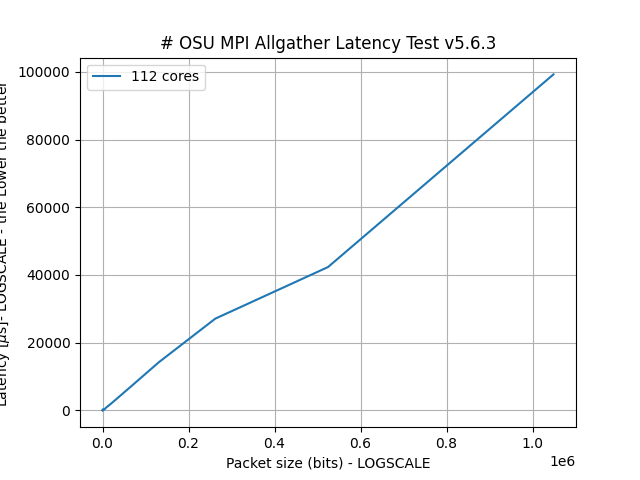
\includegraphics[width=\linewidth]{image/hardware_benchmarks/osu_benchmark/MPI_Allgather_Latency.png}
\caption{MPI\_Allgather\_Latency OSU test.}
\label{fig:MPI_Allgather_Latency.}
\end{figure}


\begin{figure}[H]
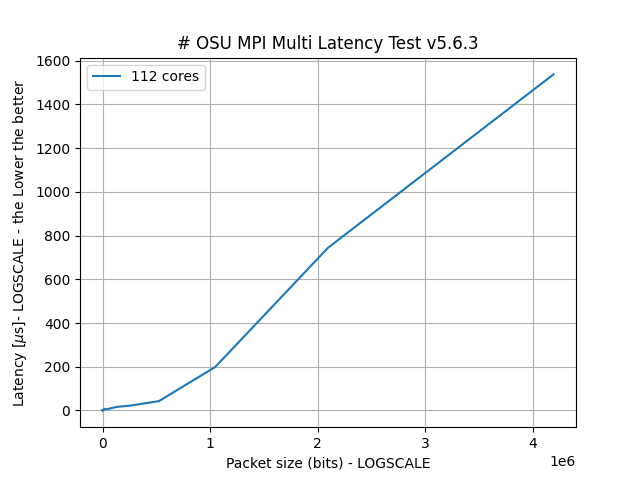
\includegraphics[width=\linewidth]{image/hardware_benchmarks/osu_benchmark/MPI_Multi_Latency.png}
\caption{MPI\_Multi\_Latency OSU test.}
\label{fig:MPI_Multi_Latency.}
\end{figure}


\begin{figure}[H]
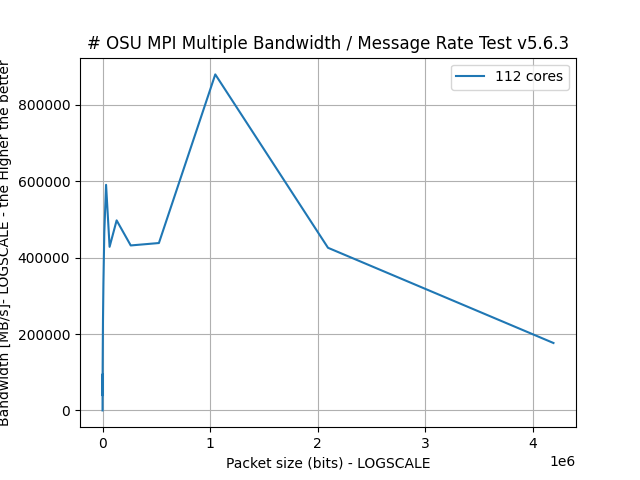
\includegraphics[width=\linewidth]{image/hardware_benchmarks/osu_benchmark/MPI_Multiple_Bandwidth_Message_Rate.png}
\caption{MPI\_Multiple\_Bandwidth\_Message\_Rate OSU test.}
\label{fig:MPI_Multiple_Bandwidth_Message_Rate.}
\end{figure}

\subsection{STREAM Benchmark}
The STREAM benchmark is a simple synthetic benchmark program that measures sustainable memory bandwidth (in $MB/s$) and the corresponding computation rate for simple vector kernels.
Computer cpus are getting faster much more quickly than computer memory systems. As this progresses, more and more programs will be limited in performance by the memory bandwidth of the system, rather than by the computational performance of the cpu.
As an extreme example, several current high-end machines run simple arithmetic kernels for out-of-cache operands at 4-5\% of their rated peak speeds --- that means that they are spending 95-96\% of their time idle and waiting for cache misses to be satisfied.
The STREAM benchmark is specifically designed to work with datasets much larger than the available cache on any given system, so that the results are (presumably) more indicative of the performance of very large, vector style applications. 


\begin{figure}[H]
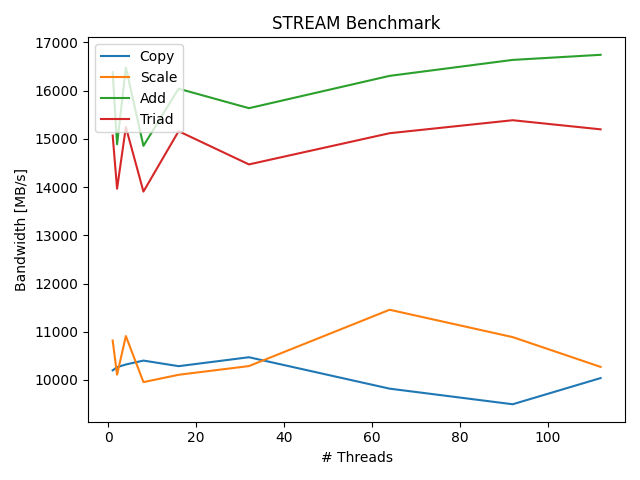
\includegraphics[width=\linewidth]{image/hardware_benchmarks/stream_benchmark/ecearth4.png}
\caption{STREAM benchmark}
\label{fig:ecearth4.}
\end{figure}

\clearpage
\section{Scalability}
The Strong Scaling member consists on running a set of tests with an increasing number of processors on the same experiment configuration. This member is evaluated by the speed of the model (SYPD). 

In the best case scenario we except that the speed of the model increases proportionally to the added number of resources with respect to the base case (the base case being the case with a lower number of resources). This perfect case can be seen in the scalability plots with the dashed line.

The efficiency metric tells us how close the current case speed is to the perfect case, where 1 means that it scales linear, lower than 1, worse than expected and bigger that 1 better than expected, and is computed by current-case-speed * current-case- base-case-speed.

The speedup metric just reports how much faster the current case is with respect to the base case.

\begin{table}[H]
\centering
\caption{Cases processors configuration}
\csvautobooktabular{csv/scalability/cases_info.csv}
\end{table}


\begin{table}[H]
\centering
\caption{Scalability table for ECEARTH4.}
\csvautobooktabular{csv/scalability/BENCH_scaling.csv}
\end{table}


\begin{figure}[H]
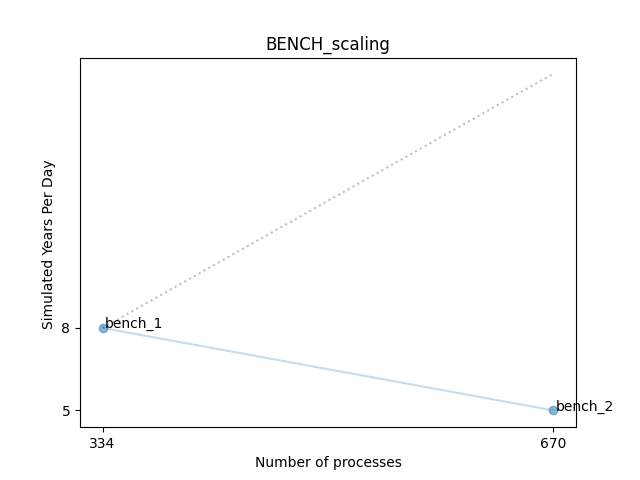
\includegraphics[width=\linewidth]{image/scalability/BENCH_scaling.png}
\caption{Scalability plot for ECEARTH4.}
\label{fig:BENCH_scaling.}
\end{figure}

\subsection{NEMO Scalability}

\begin{table}[H]
\centering
\caption{Scalability table for NEMO.}
\csvautobooktabular{csv/scalability/nemo_scalability/nemo_BENCH_scaling.csv}
\end{table}


\begin{figure}[H]
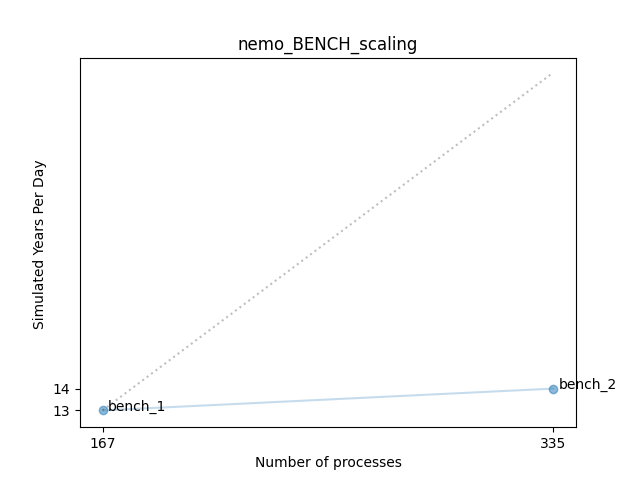
\includegraphics[width=\linewidth]{image/scalability/nemo_scalability/nemo_BENCH_scaling.png}
\caption{Scalability plot for NEMO.}
\label{fig:nemo_BENCH_scaling.}
\end{figure}

\subsection{OIFS Scalability}

\begin{table}[H]
\centering
\caption{Scalability table for OIFS.}
\csvautobooktabular{csv/scalability/oifs_scalability/oifs_BENCH_scaling.csv}
\end{table}


\begin{figure}[H]
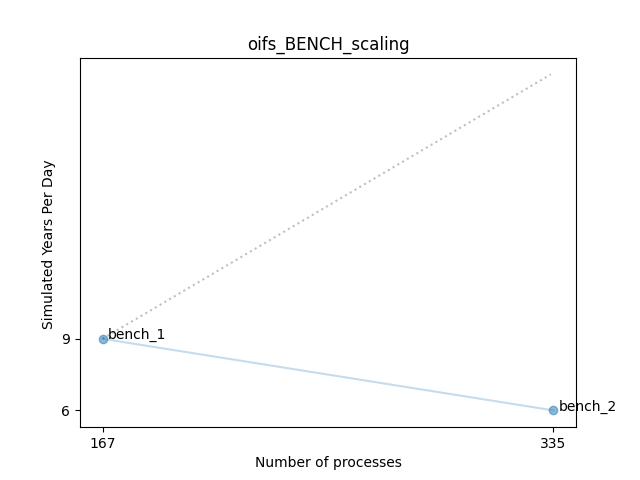
\includegraphics[width=\linewidth]{image/scalability/oifs_scalability/oifs_BENCH_scaling.png}
\caption{Scalability plot for OIFS.}
\label{fig:oifs_BENCH_scaling.}
\end{figure}

\subsection{Coupling}
\subsubsection{bench\_1}

\begin{table}[H]
\centering
\caption{Lucia results summary.}
\csvautobooktabular{csv/scalability/coupling/coupling/summary.csv}
\end{table}


\begin{figure}[H]
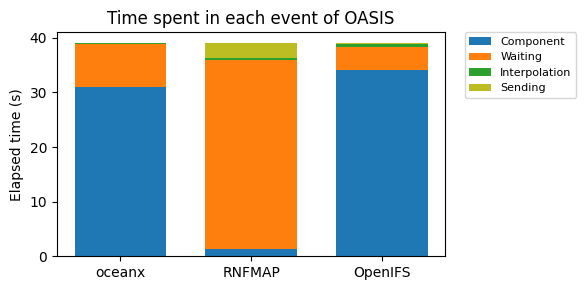
\includegraphics[width=\linewidth]{image/scalability/coupling/coupling/stacked_events.png}
\caption{Components' coupling stacked events.}
\label{fig:stacked_events.}
\end{figure}

\subsubsection{bench\_2}

\begin{table}[H]
\centering
\caption{Lucia results summary.}
\csvautobooktabular{csv/scalability/coupling/coupling/ca9c671ea8f880c476cb8756dae5630d5e36fcac1ceff97c339e88d13f66cce6_summary.csv}
\end{table}


\begin{figure}[H]
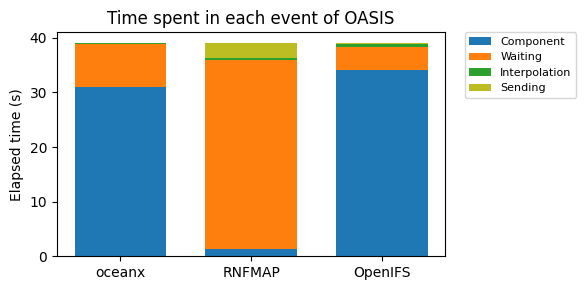
\includegraphics[width=\linewidth]{image/scalability/coupling/coupling/stacked_events.png}
\caption{Components' coupling stacked events.}
\label{fig:stacked_events.}
\end{figure}

\clearpage
\section{Tracing}

\begin{table}[H]
\centering
\caption{Test configuration.}
\csvautobooktabular{csv/tracing/test_info.csv}
\end{table}

\subsection{Functions detailed report}
This section contains, for each function of the code, a series of tables that include few key metrics that can help us to see whether the different functions scale well or not and which could be the most important factor, communication or computation.


\begin{table}[H]
\centering
\caption{Cases processors configuration.}
\csvautobooktabular{csv/tracing/functions_detailed_report/cases_info.csv}
\end{table}

\subsubsection{Most expensive function summary}

\begin{table}[H]
\centering
\caption{Most time-consuming functions for the whole model.}
\resizebox{1\textwidth}{!}{
\csvautobooktabular{csv/tracing/functions_detailed_report/functions_detailed_report/most_expensive_function_summary.csv}
}
\end{table}

\subsection{NEMO Model Factors}
This section contains performance metrics generated from a set of Paraver traces using the modelfactors tool. Comparing traces produced with a different number of resources it analyzes the evolution of communication and computation aspects of the code. 


\begin{figure}[H]
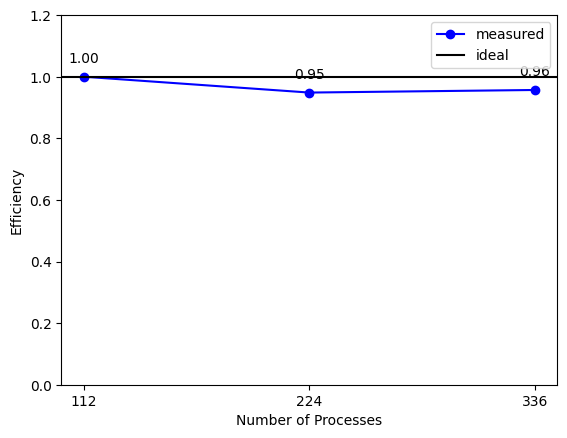
\includegraphics[width=\linewidth]{image/tracing/nemo_model_factors/efficiency-matplot.png}
\caption{Nemo modelfactors efficiency.}
\label{fig:efficiency-matplot.}
\end{figure}


\begin{figure}[H]
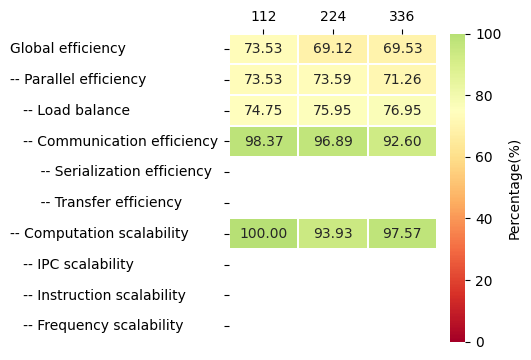
\includegraphics[width=\linewidth]{image/tracing/nemo_model_factors/efficiency_table-matplot.png}
\caption{Nemo modelfactors efficiency\_table.}
\label{fig:efficiency_table-matplot.}
\end{figure}


\begin{figure}[H]
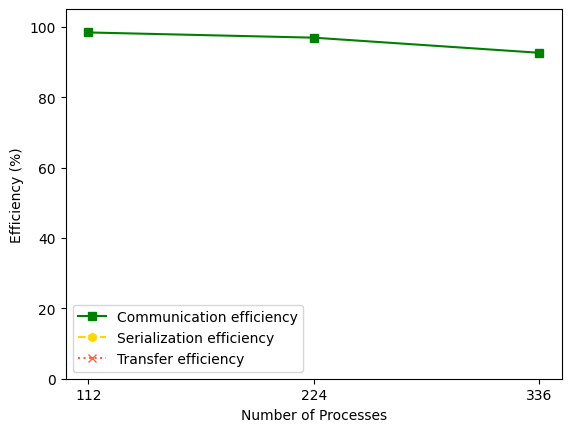
\includegraphics[width=\linewidth]{image/tracing/nemo_model_factors/modelfactors-comm-matplot.png}
\caption{Nemo modelfactors comm.}
\label{fig:modelfactors-comm-matplot.}
\end{figure}


\begin{figure}[H]
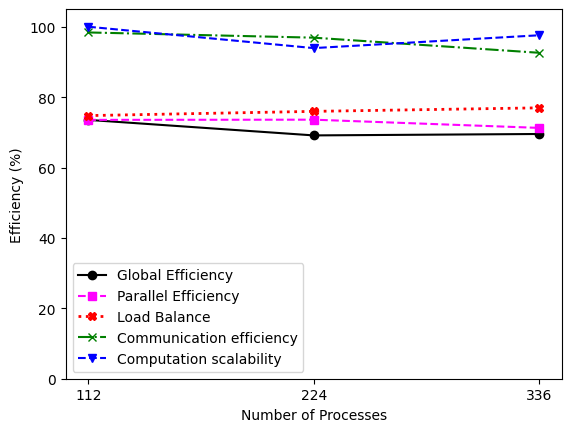
\includegraphics[width=\linewidth]{image/tracing/nemo_model_factors/modelfactors-matplot.png}
\caption{Nemo modelfactors.}
\label{fig:modelfactors-matplot.}
\end{figure}


\begin{figure}[H]
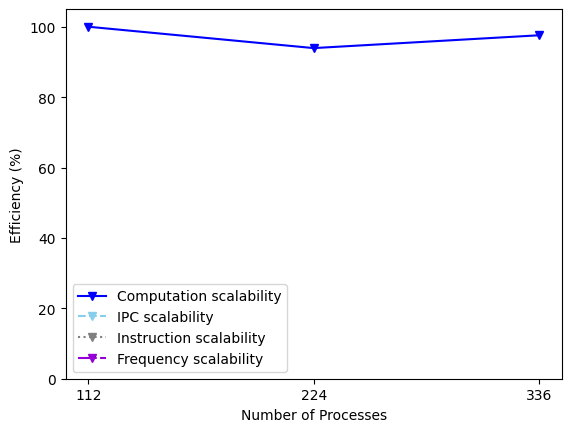
\includegraphics[width=\linewidth]{image/tracing/nemo_model_factors/modelfactors-scale-matplot.png}
\caption{Nemo modelfactors scale.}
\label{fig:modelfactors-scale-matplot.}
\end{figure}


\begin{figure}[H]
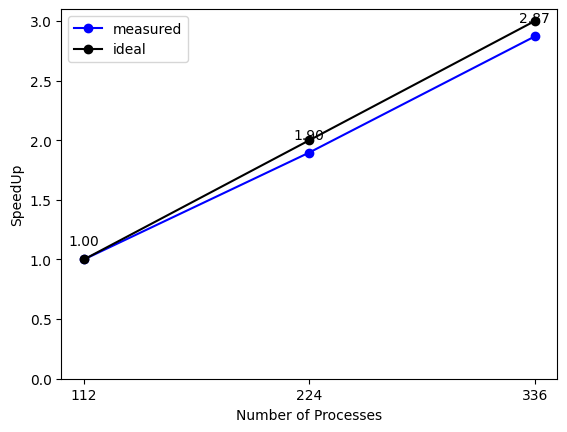
\includegraphics[width=\linewidth]{image/tracing/nemo_model_factors/speedup-matplot.png}
\caption{Nemo modelfactors speedup.}
\label{fig:speedup-matplot.}
\end{figure}

\subsection{OIFS Model Factors}
This section contains performance metrics generated from a set of Paraver traces using the modelfactors tool. Comparing traces produced with a different number of resources it analyzes the evolution of communication and computation aspects of the code. 


\begin{figure}[H]
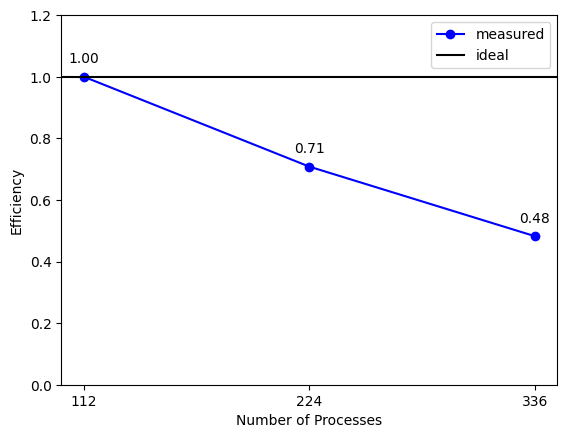
\includegraphics[width=\linewidth]{image/tracing/oifs_model_factors/efficiency-matplot.png}
\caption{Oifs modelfactors efficiency.}
\label{fig:efficiency-matplot.}
\end{figure}


\begin{figure}[H]
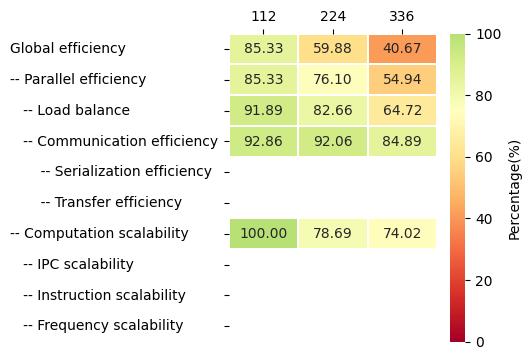
\includegraphics[width=\linewidth]{image/tracing/oifs_model_factors/efficiency_table-matplot.png}
\caption{Oifs modelfactors efficiency\_table.}
\label{fig:efficiency_table-matplot.}
\end{figure}


\begin{figure}[H]
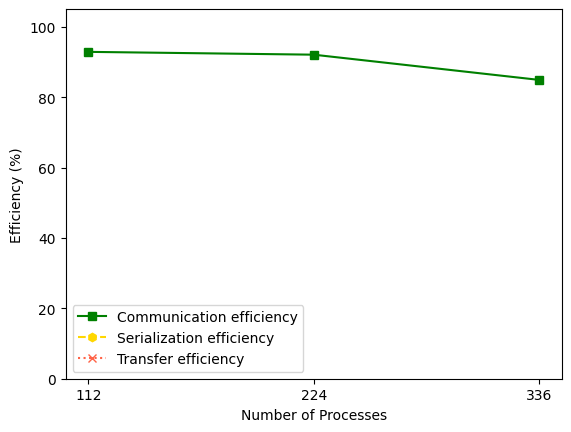
\includegraphics[width=\linewidth]{image/tracing/oifs_model_factors/modelfactors-comm-matplot.png}
\caption{Oifs modelfactors comm.}
\label{fig:modelfactors-comm-matplot.}
\end{figure}


\begin{figure}[H]
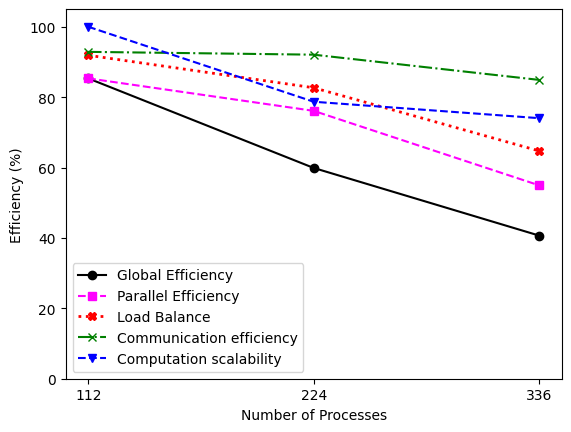
\includegraphics[width=\linewidth]{image/tracing/oifs_model_factors/modelfactors-matplot.png}
\caption{Oifs modelfactors.}
\label{fig:modelfactors-matplot.}
\end{figure}


\begin{figure}[H]
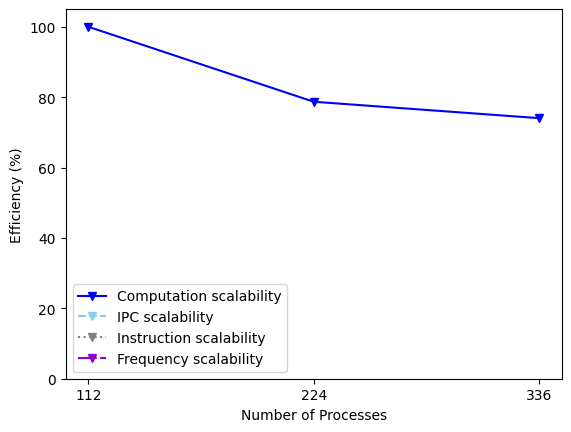
\includegraphics[width=\linewidth]{image/tracing/oifs_model_factors/modelfactors-scale-matplot.png}
\caption{Oifs modelfactors scale.}
\label{fig:modelfactors-scale-matplot.}
\end{figure}


\begin{figure}[H]
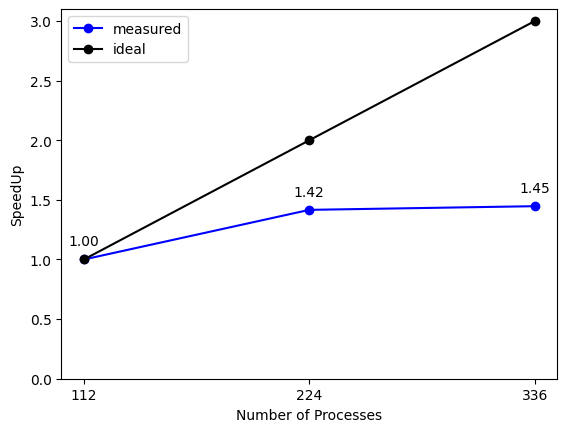
\includegraphics[width=\linewidth]{image/tracing/oifs_model_factors/speedup-matplot.png}
\caption{Oifs modelfactors speedup.}
\label{fig:speedup-matplot.}
\end{figure}

\subsection{NEMO MPI Call Profile}

\begin{landscape}
\begin{table}[H]
\centering
\caption{trace\_1 case MPI Call profile.}
\resizebox{1.5\textwidth}{!}{
\csvautobooktabular{csv/tracing/nemo_mpi_call_profile/nemo-trace_1-MPIcallprofile.csv}
}
\end{table}


\begin{table}[H]
\centering
\caption{trace\_2 case MPI Call profile.}
\resizebox{1.5\textwidth}{!}{
\csvautobooktabular{csv/tracing/nemo_mpi_call_profile/nemo-trace_2-MPIcallprofile.csv}
}
\end{table}


\begin{table}[H]
\centering
\caption{trace\_3 case MPI Call profile.}
\resizebox{1.5\textwidth}{!}{
\csvautobooktabular{csv/tracing/nemo_mpi_call_profile/nemo-trace_3-MPIcallprofile.csv}
}
\end{table}

\end{landscape}
\subsection{OIFS MPI Call Profile}

\begin{landscape}
\begin{table}[H]
\centering
\caption{trace\_1 case MPI Call profile.}
\resizebox{1.5\textwidth}{!}{
\csvautobooktabular{csv/tracing/oifs_mpi_call_profile/oifs-trace_1-MPIcallprofile.csv}
}
\end{table}


\begin{table}[H]
\centering
\caption{trace\_2 case MPI Call profile.}
\resizebox{1.5\textwidth}{!}{
\csvautobooktabular{csv/tracing/oifs_mpi_call_profile/oifs-trace_2-MPIcallprofile.csv}
}
\end{table}


\begin{table}[H]
\centering
\caption{trace\_3 case MPI Call profile.}
\resizebox{1.5\textwidth}{!}{
\csvautobooktabular{csv/tracing/oifs_mpi_call_profile/oifs-trace_3-MPIcallprofile.csv}
}
\end{table}

\end{landscape}
\subsection{NEMO Functions detailed report}
\subsubsection{Most expensive function summary}

\begin{table}[H]
\centering
\caption{Most time-consuming functions for NEMO.}
\resizebox{1\textwidth}{!}{
\csvautobooktabular{csv/tracing/nemo_functions_detailed_report/nemo_functions_detailed_report/nemo_most_expensive_function_summary.csv}
}
\end{table}

\subsubsection{PAPI counters plots}

\begin{figure}[H]
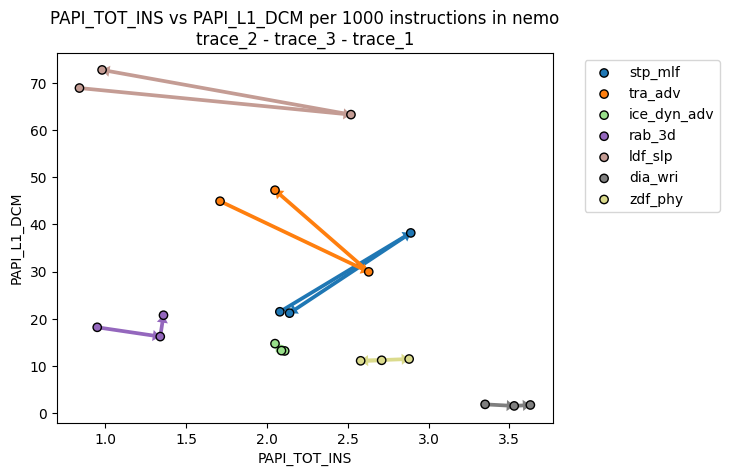
\includegraphics[width=\linewidth]{image/tracing/nemo_functions_detailed_report/nemo_functions_detailed_report/nemo-PAPI_TOT_INS-PAPI_L1_DCM.png}
\caption{PAPI\_TOT\_INS vs PAPI\_L1\_DCM counters plot for nemo.}
\label{fig:nemo-PAPI_TOT_INS-PAPI_L1_DCM.}
\end{figure}


\begin{figure}[H]
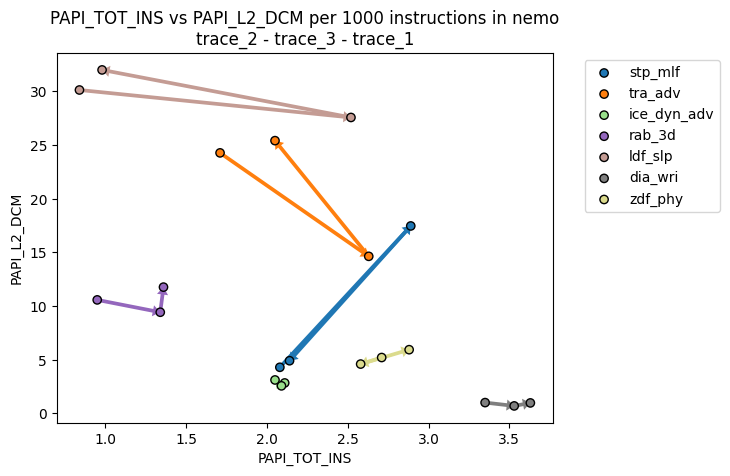
\includegraphics[width=\linewidth]{image/tracing/nemo_functions_detailed_report/nemo_functions_detailed_report/nemo-PAPI_TOT_INS-PAPI_L2_DCM.png}
\caption{PAPI\_TOT\_INS vs PAPI\_L2\_DCM counters plot for nemo.}
\label{fig:nemo-PAPI_TOT_INS-PAPI_L2_DCM.}
\end{figure}


\begin{figure}[H]
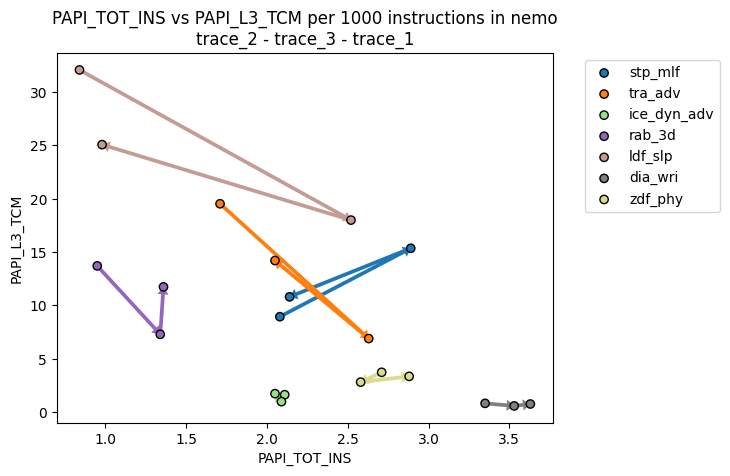
\includegraphics[width=\linewidth]{image/tracing/nemo_functions_detailed_report/nemo_functions_detailed_report/nemo-PAPI_TOT_INS-PAPI_L3_TCM.png}
\caption{PAPI\_TOT\_INS vs PAPI\_L3\_TCM counters plot for nemo.}
\label{fig:nemo-PAPI_TOT_INS-PAPI_L3_TCM.}
\end{figure}


\begin{figure}[H]
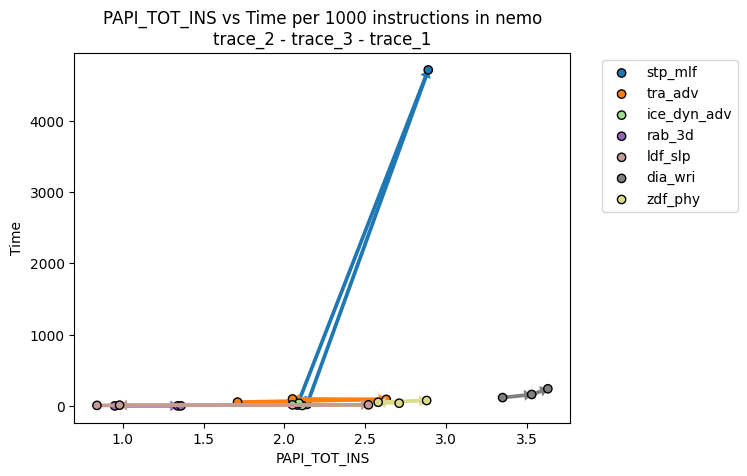
\includegraphics[width=\linewidth]{image/tracing/nemo_functions_detailed_report/nemo_functions_detailed_report/nemo-PAPI_TOT_INS-Time.png}
\caption{PAPI\_TOT\_INS vs Time counters plot for nemo.}
\label{fig:nemo-PAPI_TOT_INS-Time.}
\end{figure}


\begin{figure}[H]
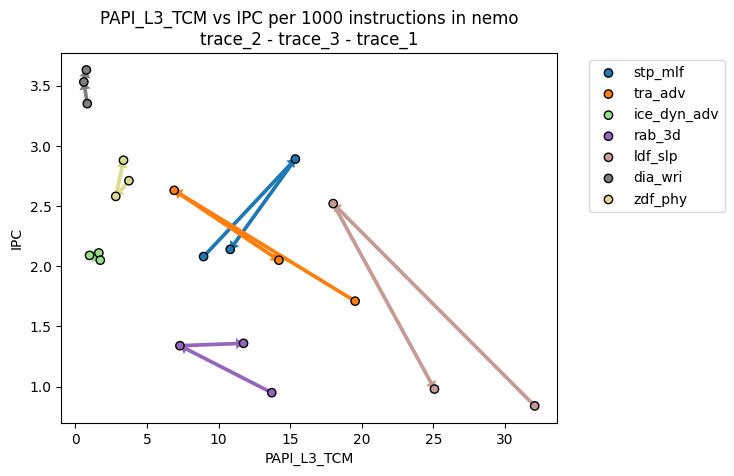
\includegraphics[width=\linewidth]{image/tracing/nemo_functions_detailed_report/nemo_functions_detailed_report/nemo-PAPI_L3_TCM-IPC.png}
\caption{PAPI\_L3\_TCM vs IPC counters plot for nemo.}
\label{fig:nemo-PAPI_L3_TCM-IPC.}
\end{figure}

\subsubsection{nemo\_dia\_wri}

\begin{table}[H]
\centering
\caption{nemo\_dia\_wri scalability.}
\csvautobooktabular{csv/tracing/nemo_functions_detailed_report/nemo_functions_detailed_report/nemo_dia_wri.csv}
\end{table}


\begin{table}[H]
\centering
\caption{nemo\_dia\_wri MPI scalability.}
\csvautobooktabular{csv/tracing/nemo_functions_detailed_report/nemo_functions_detailed_report/fe46228012a614d94818b602d05d33a5729583040c42f9fef7222d84344997ef_nemo_dia_wri.csv}
\end{table}


\begin{table}[H]
\centering
\caption{nemo\_dia\_wri counters scalability.}
\csvautobooktabular{csv/tracing/nemo_functions_detailed_report/nemo_functions_detailed_report/4e9a9cad5cba6178051ebbd7024e2f5ccef0b74f72839db32b6fee795b73d12e_nemo_dia_wri.csv}
\end{table}

\subsubsection{nemo\_ice\_dyn\_adv}

\begin{table}[H]
\centering
\caption{nemo\_ice\_dyn\_adv scalability.}
\csvautobooktabular{csv/tracing/nemo_functions_detailed_report/nemo_functions_detailed_report/nemo_ice_dyn_adv.csv}
\end{table}


\begin{table}[H]
\centering
\caption{nemo\_ice\_dyn\_adv MPI scalability.}
\csvautobooktabular{csv/tracing/nemo_functions_detailed_report/nemo_functions_detailed_report/8fc2a08e5ad6f6c1884e1d97fdf9e5cbe565feadf41cf8cf2130da917967e3bf_nemo_ice_dyn_adv.csv}
\end{table}


\begin{table}[H]
\centering
\caption{nemo\_ice\_dyn\_adv counters scalability.}
\csvautobooktabular{csv/tracing/nemo_functions_detailed_report/nemo_functions_detailed_report/06b2305907761e4ce08c49d408946f093ff0427c265d786f6b8ab6750ac9aaea_nemo_ice_dyn_adv.csv}
\end{table}

\subsubsection{nemo\_ldf\_slp}

\begin{table}[H]
\centering
\caption{nemo\_ldf\_slp scalability.}
\csvautobooktabular{csv/tracing/nemo_functions_detailed_report/nemo_functions_detailed_report/nemo_ldf_slp.csv}
\end{table}


\begin{table}[H]
\centering
\caption{nemo\_ldf\_slp MPI scalability.}
\csvautobooktabular{csv/tracing/nemo_functions_detailed_report/nemo_functions_detailed_report/6c1227fe49a9fac8775967a87cca5931f4613ae11ff19a077e504dc0884e7563_nemo_ldf_slp.csv}
\end{table}


\begin{table}[H]
\centering
\caption{nemo\_ldf\_slp counters scalability.}
\csvautobooktabular{csv/tracing/nemo_functions_detailed_report/nemo_functions_detailed_report/6f9811811a6221497883f65a1a14750febc47efbbbd3657b185abe8bdb8cb623_nemo_ldf_slp.csv}
\end{table}

\subsubsection{nemo\_rab\_3d}

\begin{table}[H]
\centering
\caption{nemo\_rab\_3d scalability.}
\csvautobooktabular{csv/tracing/nemo_functions_detailed_report/nemo_functions_detailed_report/nemo_rab_3d.csv}
\end{table}

\subsubsection{nemo\_stp\_mlf}

\begin{table}[H]
\centering
\caption{nemo\_stp\_mlf scalability.}
\csvautobooktabular{csv/tracing/nemo_functions_detailed_report/nemo_functions_detailed_report/nemo_stp_mlf.csv}
\end{table}


\begin{table}[H]
\centering
\caption{nemo\_stp\_mlf MPI scalability.}
\csvautobooktabular{csv/tracing/nemo_functions_detailed_report/nemo_functions_detailed_report/4b9a536c33ecfaab71d0da13892cd32ad9d151bceb01c86a115d3dc49724763d_nemo_stp_mlf.csv}
\end{table}


\begin{table}[H]
\centering
\caption{nemo\_stp\_mlf counters scalability.}
\csvautobooktabular{csv/tracing/nemo_functions_detailed_report/nemo_functions_detailed_report/1f8c80079d48205d795959661ac6d6a725cb9340721c96b5faa77da0106ac33b_nemo_stp_mlf.csv}
\end{table}

\subsubsection{nemo\_tra\_adv}

\begin{table}[H]
\centering
\caption{nemo\_tra\_adv scalability.}
\csvautobooktabular{csv/tracing/nemo_functions_detailed_report/nemo_functions_detailed_report/nemo_tra_adv.csv}
\end{table}


\begin{table}[H]
\centering
\caption{nemo\_tra\_adv MPI scalability.}
\csvautobooktabular{csv/tracing/nemo_functions_detailed_report/nemo_functions_detailed_report/c6a1c5ee3c9e6cbf1a642bb1bfa0f2492bf9fd251af12d34137658dbb0eefdf6_nemo_tra_adv.csv}
\end{table}


\begin{table}[H]
\centering
\caption{nemo\_tra\_adv counters scalability.}
\csvautobooktabular{csv/tracing/nemo_functions_detailed_report/nemo_functions_detailed_report/a47ca0b784ea1292dce004b4b7bdeb558be736c7ed4f3761c326fddb0926ace5_nemo_tra_adv.csv}
\end{table}

\subsubsection{nemo\_zdf\_phy}

\begin{table}[H]
\centering
\caption{nemo\_zdf\_phy scalability.}
\csvautobooktabular{csv/tracing/nemo_functions_detailed_report/nemo_functions_detailed_report/nemo_zdf_phy.csv}
\end{table}


\begin{table}[H]
\centering
\caption{nemo\_zdf\_phy MPI scalability.}
\csvautobooktabular{csv/tracing/nemo_functions_detailed_report/nemo_functions_detailed_report/1a5defec8f37555d10b77e04589de900a17475c26d74ea22f46c87da10d36ae9_nemo_zdf_phy.csv}
\end{table}


\begin{table}[H]
\centering
\caption{nemo\_zdf\_phy counters scalability.}
\csvautobooktabular{csv/tracing/nemo_functions_detailed_report/nemo_functions_detailed_report/d3875eeb769f17f6c9f22f12908b45e27a6b624fb170802d7d64469b8b70c7d5_nemo_zdf_phy.csv}
\end{table}

\subsection{OIFS Functions detailed report}
\subsubsection{Most expensive function summary}

\begin{table}[H]
\centering
\caption{Most time-consuming functions for OIFS.}
\resizebox{1\textwidth}{!}{
\csvautobooktabular{csv/tracing/oifs_functions_detailed_report/oifs_functions_detailed_report/oifs_most_expensive_function_summary.csv}
}
\end{table}

\subsubsection{PAPI counters plots}

\begin{figure}[H]
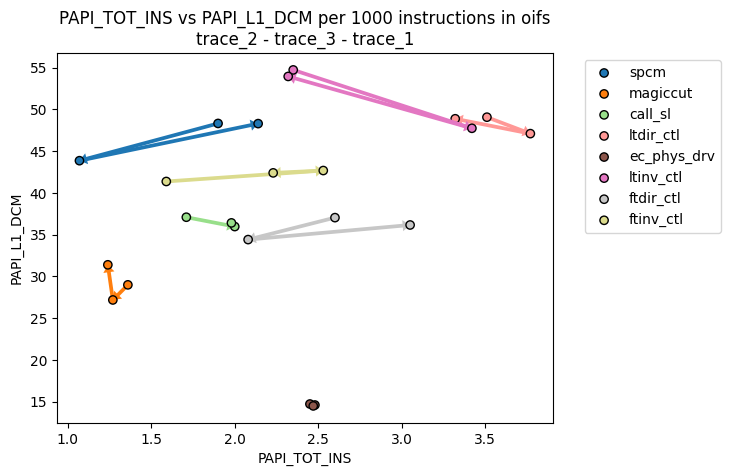
\includegraphics[width=\linewidth]{image/tracing/oifs_functions_detailed_report/oifs_functions_detailed_report/oifs-PAPI_TOT_INS-PAPI_L1_DCM.png}
\caption{PAPI\_TOT\_INS vs PAPI\_L1\_DCM counters plot for oifs.}
\label{fig:oifs-PAPI_TOT_INS-PAPI_L1_DCM.}
\end{figure}


\begin{figure}[H]
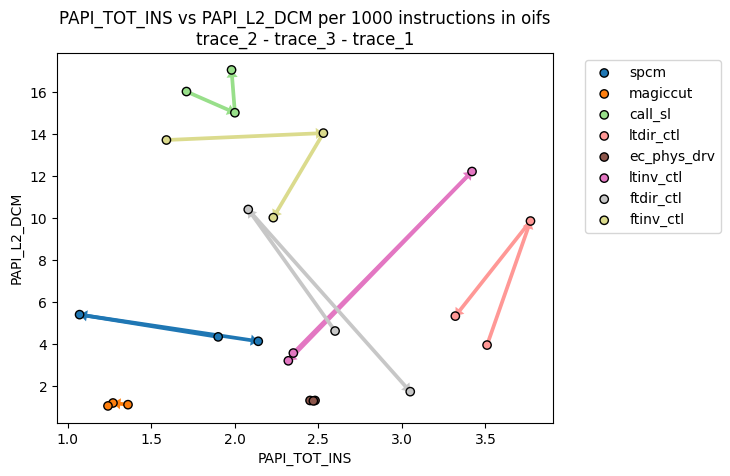
\includegraphics[width=\linewidth]{image/tracing/oifs_functions_detailed_report/oifs_functions_detailed_report/oifs-PAPI_TOT_INS-PAPI_L2_DCM.png}
\caption{PAPI\_TOT\_INS vs PAPI\_L2\_DCM counters plot for oifs.}
\label{fig:oifs-PAPI_TOT_INS-PAPI_L2_DCM.}
\end{figure}


\begin{figure}[H]
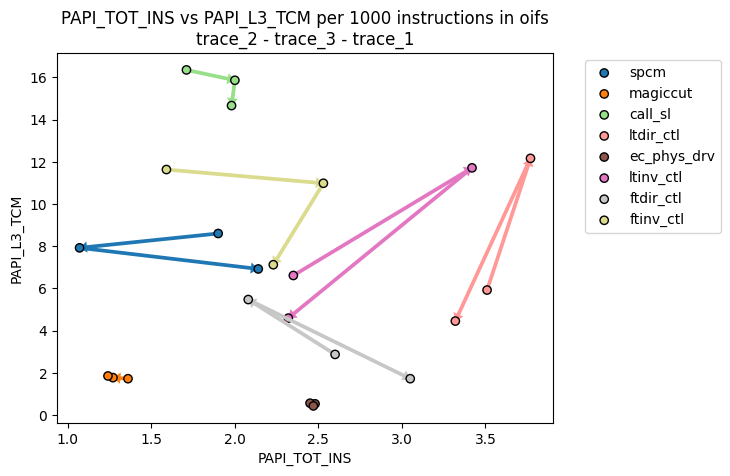
\includegraphics[width=\linewidth]{image/tracing/oifs_functions_detailed_report/oifs_functions_detailed_report/oifs-PAPI_TOT_INS-PAPI_L3_TCM.png}
\caption{PAPI\_TOT\_INS vs PAPI\_L3\_TCM counters plot for oifs.}
\label{fig:oifs-PAPI_TOT_INS-PAPI_L3_TCM.}
\end{figure}


\begin{figure}[H]
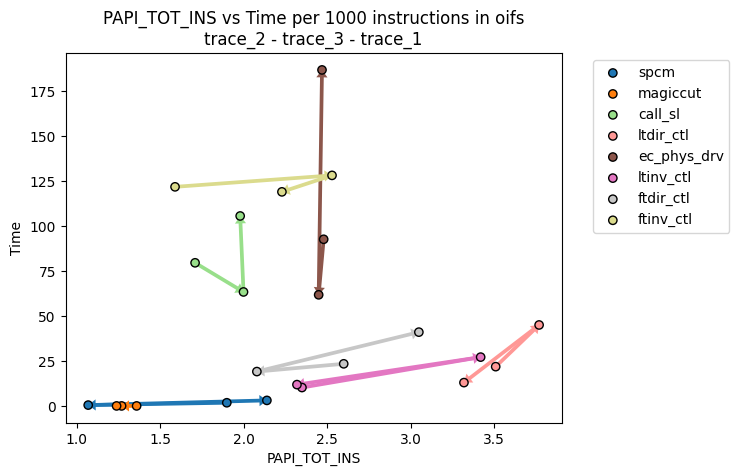
\includegraphics[width=\linewidth]{image/tracing/oifs_functions_detailed_report/oifs_functions_detailed_report/oifs-PAPI_TOT_INS-Time.png}
\caption{PAPI\_TOT\_INS vs Time counters plot for oifs.}
\label{fig:oifs-PAPI_TOT_INS-Time.}
\end{figure}


\begin{figure}[H]
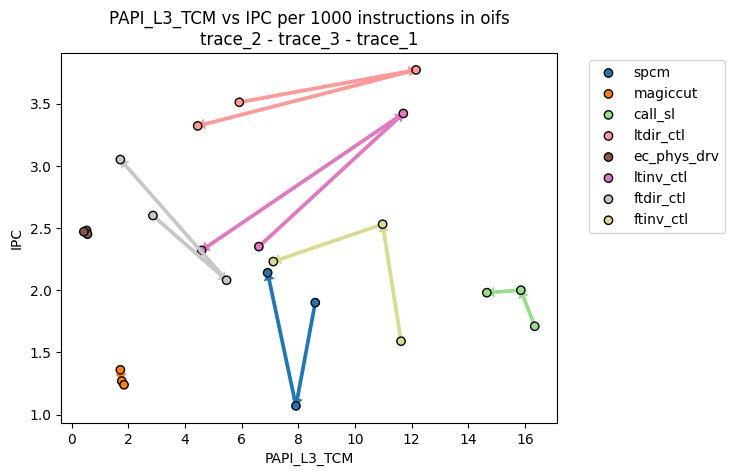
\includegraphics[width=\linewidth]{image/tracing/oifs_functions_detailed_report/oifs_functions_detailed_report/oifs-PAPI_L3_TCM-IPC.png}
\caption{PAPI\_L3\_TCM vs IPC counters plot for oifs.}
\label{fig:oifs-PAPI_L3_TCM-IPC.}
\end{figure}

\subsubsection{oifs\_call\_sl}

\begin{table}[H]
\centering
\caption{oifs\_call\_sl scalability.}
\csvautobooktabular{csv/tracing/oifs_functions_detailed_report/oifs_functions_detailed_report/oifs_call_sl.csv}
\end{table}


\begin{table}[H]
\centering
\caption{oifs\_call\_sl MPI scalability.}
\csvautobooktabular{csv/tracing/oifs_functions_detailed_report/oifs_functions_detailed_report/0b3ac44203165ba4395d81095a3764a92c81fdc5354edb5f8afa06c81caec3c6_oifs_call_sl.csv}
\end{table}


\begin{table}[H]
\centering
\caption{oifs\_call\_sl counters scalability.}
\csvautobooktabular{csv/tracing/oifs_functions_detailed_report/oifs_functions_detailed_report/3489ddd5a5f13d38ef6590191d8f641dd5ab70a76db3fabc71c2559924eabc06_oifs_call_sl.csv}
\end{table}

\subsubsection{oifs\_ec\_phys\_drv}

\begin{table}[H]
\centering
\caption{oifs\_ec\_phys\_drv scalability.}
\csvautobooktabular{csv/tracing/oifs_functions_detailed_report/oifs_functions_detailed_report/oifs_ec_phys_drv.csv}
\end{table}


\begin{table}[H]
\centering
\caption{oifs\_ec\_phys\_drv MPI scalability.}
\csvautobooktabular{csv/tracing/oifs_functions_detailed_report/oifs_functions_detailed_report/306f255e829c5970e1aebead40ff4ef023c974efc00aaba388eaa2380830b8b8_oifs_ec_phys_drv.csv}
\end{table}


\begin{table}[H]
\centering
\caption{oifs\_ec\_phys\_drv counters scalability.}
\csvautobooktabular{csv/tracing/oifs_functions_detailed_report/oifs_functions_detailed_report/90cad477ae1988c2e53a52137d2f28c0ebda51deca1be0355c8c032098da46e3_oifs_ec_phys_drv.csv}
\end{table}

\subsubsection{oifs\_ftdir\_ctl}

\begin{table}[H]
\centering
\caption{oifs\_ftdir\_ctl scalability.}
\csvautobooktabular{csv/tracing/oifs_functions_detailed_report/oifs_functions_detailed_report/oifs_ftdir_ctl.csv}
\end{table}


\begin{table}[H]
\centering
\caption{oifs\_ftdir\_ctl MPI scalability.}
\csvautobooktabular{csv/tracing/oifs_functions_detailed_report/oifs_functions_detailed_report/b1fae6aaa156a839eb33669f25ef57ca03652f1807200f497c8b7d18acf213f4_oifs_ftdir_ctl.csv}
\end{table}


\begin{table}[H]
\centering
\caption{oifs\_ftdir\_ctl counters scalability.}
\csvautobooktabular{csv/tracing/oifs_functions_detailed_report/oifs_functions_detailed_report/22e0f294709696803b8642244b135b134114d606f23d0776c22a68c54f0bf9db_oifs_ftdir_ctl.csv}
\end{table}

\subsubsection{oifs\_ftinv\_ctl}

\begin{table}[H]
\centering
\caption{oifs\_ftinv\_ctl scalability.}
\csvautobooktabular{csv/tracing/oifs_functions_detailed_report/oifs_functions_detailed_report/oifs_ftinv_ctl.csv}
\end{table}


\begin{table}[H]
\centering
\caption{oifs\_ftinv\_ctl MPI scalability.}
\csvautobooktabular{csv/tracing/oifs_functions_detailed_report/oifs_functions_detailed_report/b714f8086161fc3f27c67b50622f56d16b26f7fc6a1b14e5d1c79d4ddedb2e07_oifs_ftinv_ctl.csv}
\end{table}


\begin{table}[H]
\centering
\caption{oifs\_ftinv\_ctl counters scalability.}
\csvautobooktabular{csv/tracing/oifs_functions_detailed_report/oifs_functions_detailed_report/19722182b7a457bd8cd0add5faf11dc67d2f19ace23fd8b8a2f4d6649e6f82fb_oifs_ftinv_ctl.csv}
\end{table}

\subsubsection{oifs\_ltdir\_ctl}

\begin{table}[H]
\centering
\caption{oifs\_ltdir\_ctl scalability.}
\csvautobooktabular{csv/tracing/oifs_functions_detailed_report/oifs_functions_detailed_report/oifs_ltdir_ctl.csv}
\end{table}


\begin{table}[H]
\centering
\caption{oifs\_ltdir\_ctl MPI scalability.}
\csvautobooktabular{csv/tracing/oifs_functions_detailed_report/oifs_functions_detailed_report/a6a41901620b894507791e8c0e1c81bf84fc084ec267ba8f6aa9c1b3ce2d8299_oifs_ltdir_ctl.csv}
\end{table}


\begin{table}[H]
\centering
\caption{oifs\_ltdir\_ctl counters scalability.}
\csvautobooktabular{csv/tracing/oifs_functions_detailed_report/oifs_functions_detailed_report/ac203990d7fc174c4c3e11748a3576ac230bfe1bcfcb139df464ee3c21ed0234_oifs_ltdir_ctl.csv}
\end{table}

\subsubsection{oifs\_ltinv\_ctl}

\begin{table}[H]
\centering
\caption{oifs\_ltinv\_ctl scalability.}
\csvautobooktabular{csv/tracing/oifs_functions_detailed_report/oifs_functions_detailed_report/oifs_ltinv_ctl.csv}
\end{table}


\begin{table}[H]
\centering
\caption{oifs\_ltinv\_ctl MPI scalability.}
\csvautobooktabular{csv/tracing/oifs_functions_detailed_report/oifs_functions_detailed_report/82c129bbad098cfce7d2c7fcb1a1b9a213d270cb42d792e02a8de5ea7971caae_oifs_ltinv_ctl.csv}
\end{table}


\begin{table}[H]
\centering
\caption{oifs\_ltinv\_ctl counters scalability.}
\csvautobooktabular{csv/tracing/oifs_functions_detailed_report/oifs_functions_detailed_report/91759c23438817bae6f41472617f4f57037157988b1d5f31ce212aa5957f78be_oifs_ltinv_ctl.csv}
\end{table}

\subsubsection{oifs\_magiccut}

\begin{table}[H]
\centering
\caption{oifs\_magiccut scalability.}
\csvautobooktabular{csv/tracing/oifs_functions_detailed_report/oifs_functions_detailed_report/oifs_magiccut.csv}
\end{table}

\subsubsection{oifs\_spcm}

\begin{table}[H]
\centering
\caption{oifs\_spcm scalability.}
\csvautobooktabular{csv/tracing/oifs_functions_detailed_report/oifs_functions_detailed_report/oifs_spcm.csv}
\end{table}

\end{document}
